\documentclass[12pt]{article}
\usepackage{amsmath}
\usepackage{amssymb}
%\usepackage{hyperref}
\usepackage{epsfig,graphicx,amsmath}
\usepackage{amsfonts}
\usepackage{enumerate}
\usepackage{amsfonts}
\usepackage{amssymb}
\usepackage{amsthm}

\newcommand{\mb}[1]{\mbox{\boldmath$#1$}}
\newcommand{\p}{\partial}
\newcommand{\ds}{\displaystyle}
\newcommand{\beq}{\begin{eqnarray}}
\newcommand{\beqq}{\begin{eqnarray*}}
\newcommand{\eeq}{\end{eqnarray}}
\newcommand{\eeqq}{\end{eqnarray*}}
\newcommand{\eps}{\varepsilon}
\newcommand{\erf}{\mbox{erf}}
\newcommand{\erfi}{\mbox{erfi}}
\newcommand{\Ei}{\mbox{Ei}}
\newcommand{\x}{\mbox{\boldmath$x$}}
\newcommand{\Aa}{\mbox{\boldmath$A$}}
\newcommand{\rr}{\mbox{\boldmath$r$}}
\newcommand{\As}{\mbox{\boldmath$a$}}
\newcommand{\y}{\mbox{\boldmath$y$}}
\newcommand{\z}{\mbox{\boldmath$z$}}
\newcommand{\J}{\mbox{\boldmath$J$}}
\newcommand{\ET}{\mbox{\boldmath$\eta$}}
\newcommand{\n}{\mbox{\boldmath$n$}}
\newcommand{\X}{\mbox{\boldmath$X$}}
\newcommand{\Y}{\mbox{\boldmath$Y$}}
\newcommand{\Yy}{\mbox{\boldmath$y$}}
\newcommand{\Z}{\mbox{\boldmath$Z$}}
\newcommand{\w}{\mbox{\boldmath$w$}}
\newcommand{\vv}{\mbox{\boldmath$v$}}
\newcommand{\bb}{\mbox{\boldmath$b$}}
\newcommand{\Bb}{\mbox{\boldmath$b$}}
\newcommand{\B}{\mbox{\boldmath$B$}}
\newcommand{\ALPHA}{\mbox{\boldmath$\alpha$}}
\newcommand{\aaa}{\mbox{\boldmath$a$}}
\newcommand{\C}{\mbox{\boldmath$C$}}
\newcommand{\SSigma}{\mbox{\boldmath$\Sigma$}}
\newcommand{\mmu}{\mbox{\boldmath$\mu$}}
\newcommand{\IIm}{\mbox{\boldmath$I_m$}}
\newcommand{\mean}[1]{\langle #1\rangle}
\newcommand{\diffunit}{$\mu$m$^2$.s$^{-1}$}
\newcommand{\Li}{\mbox{Li}}
\newcommand{\thet}{\mbox{\boldmath$\theta$}}
\newcommand{\intR}{\int\limits_{\mathbb{R}}}
\newcommand{\intRm}{\int\limits_{\mathbb{R}^m}}
\newcommand\norm[1]{\left\lVert#1\right\rVert}
%\definecolor{red}{rgb}{1,0,0}

\usepackage{color}
\usepackage{float}
\begin{document}	
	\title{Results \& Material and methods}
	\author{Ofir Shukron \& David Holcman}
	\maketitle
	
	\section{Result section}
	To estimate the nucleosome reorganization following DNA damages, we have
	constructed a mathematical model, where redistribution can be due either to chromatin de-compaction or nucleosome sliding along the chromatin or both of them. We have used the model to assess the relative contribution of these two processes to the total DNA and nucleosome signal loss from a region of interest (ROI), a quantity which is inaccessible experimentally.
	
	The model (presented in Material and methods) follows the DNA, $D(u)$,
	and nucleosome, $H(u)$, fraction of signal loss from the ROI as a function of
	the UV dose, $u$. We have used the measured H3.3 and DNA signal loss to
	calibrate parameters of nucleosome and DNA models respectively.
	
	Using the calibrated models we have found that the relative contribution
	of nucleosome sliding to the total signal loss in the ROI is monotonically
	decreasing from 62.5\% to 56.3\% for nucleosomes and 27.3\% to 20\% for DNA loss,
	as the UV dose increases from 0 to 100 msec. The remaining percentages are
	attributed to chromatin expansion and de-compaction (see Figure \ref{fig:relatiiveContributionToLoss}).
	
	\begin{figure}[H]
		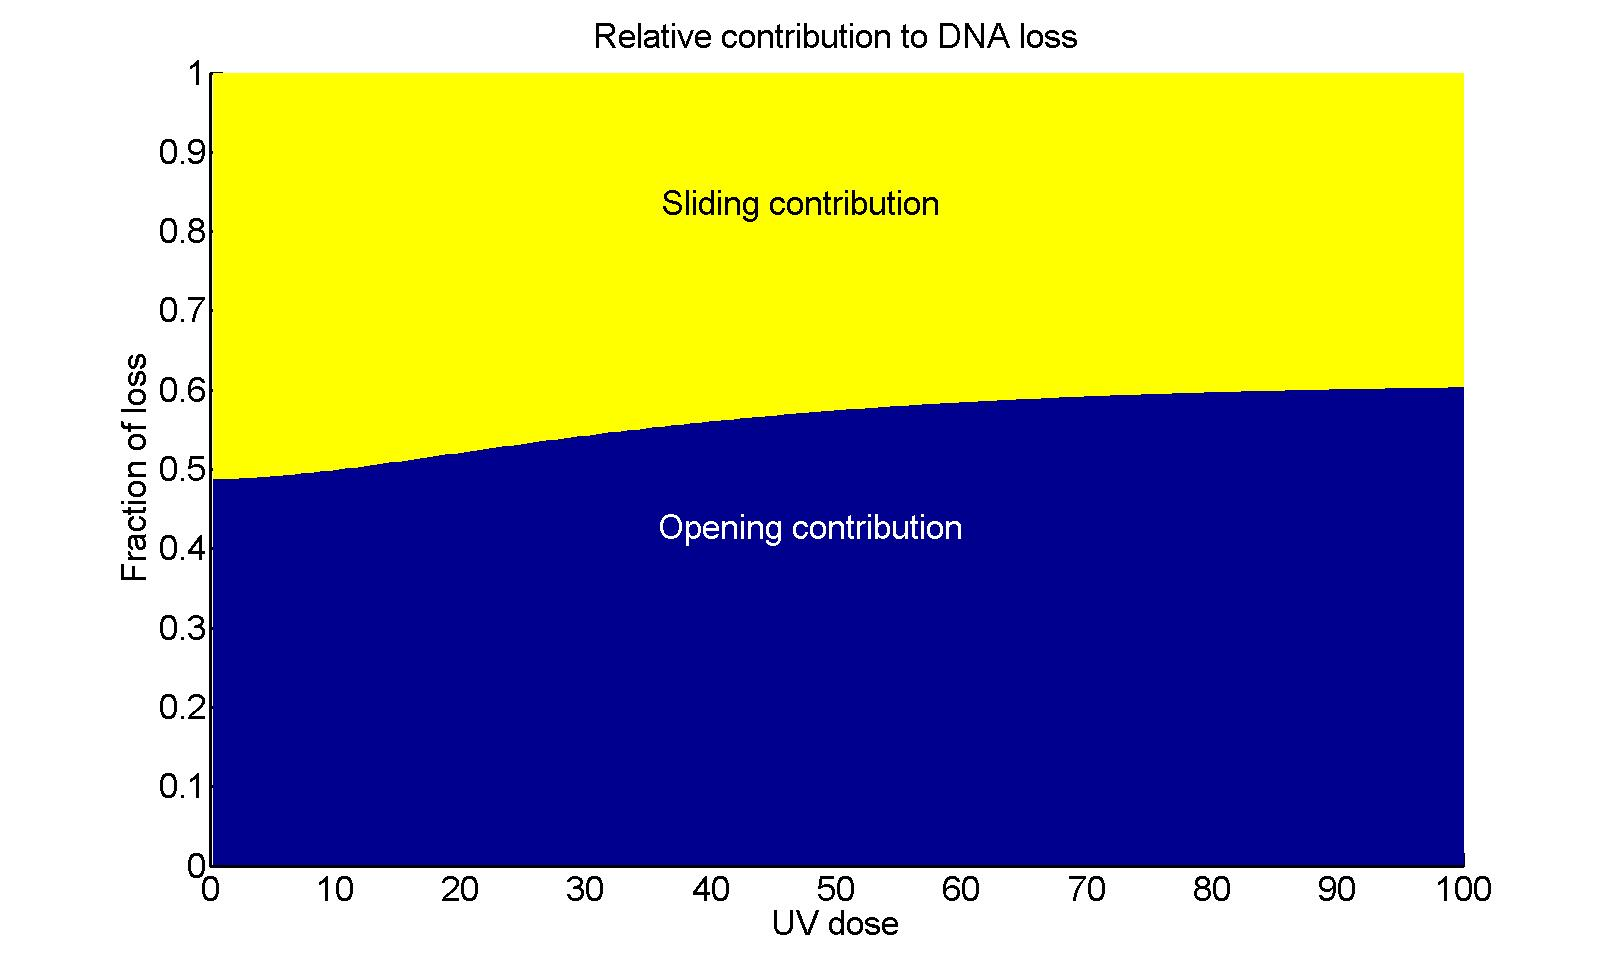
\includegraphics[width=0.5\linewidth, height=0.3\textheight]{relatiiveContributionToDNALoss}
		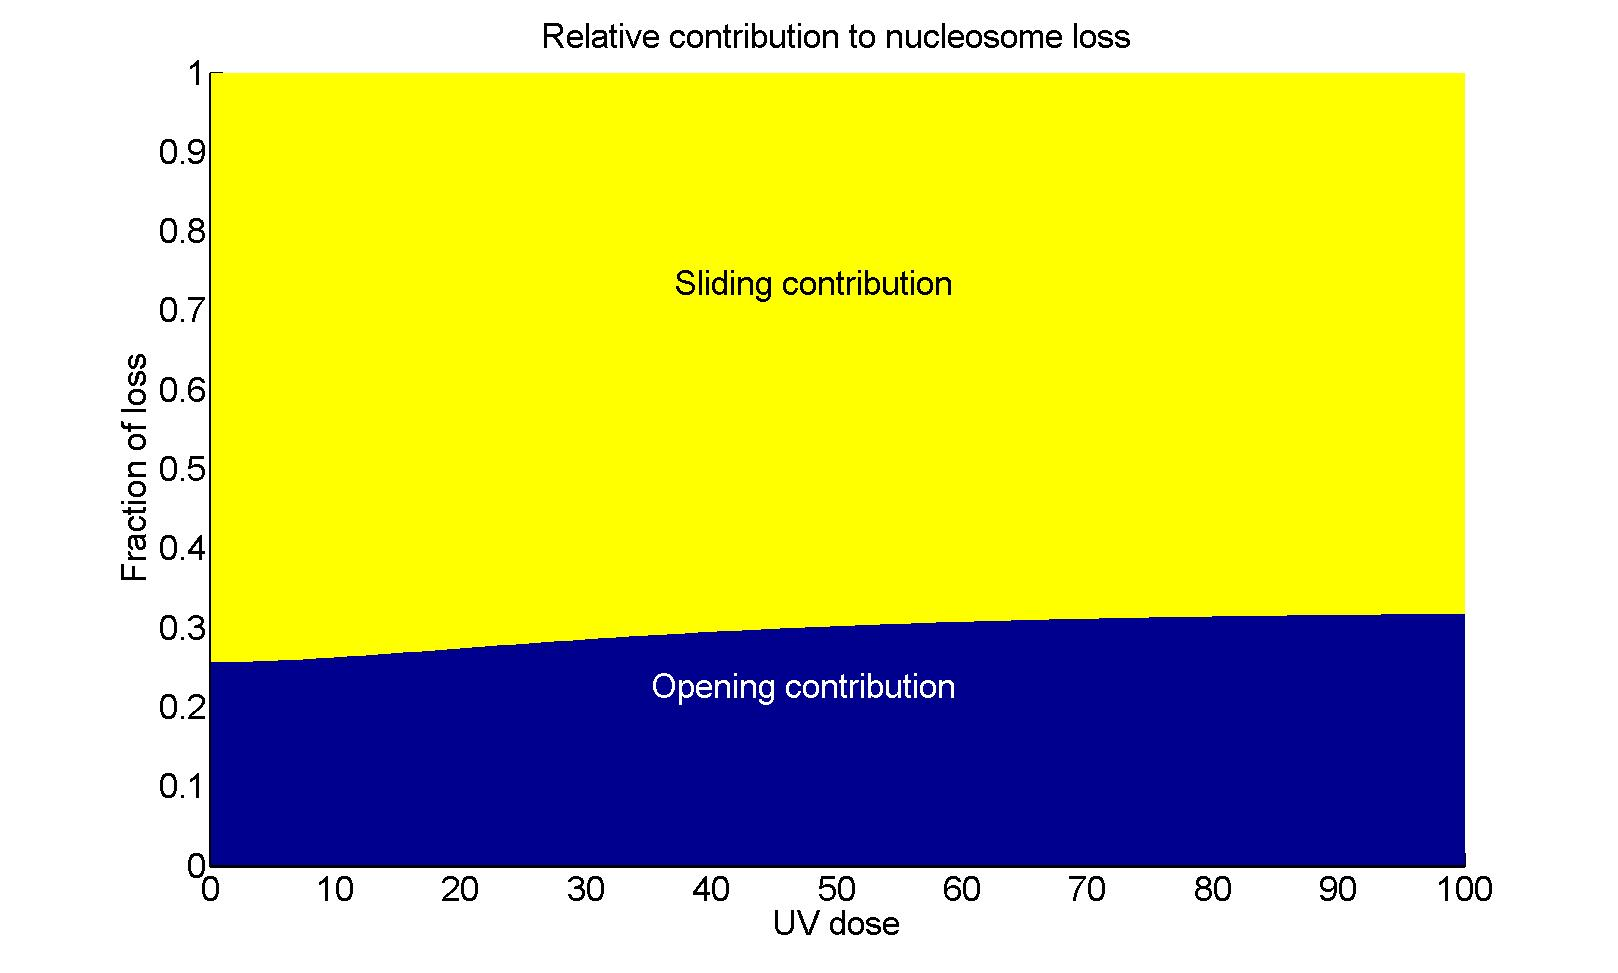
\includegraphics[width=0.5\linewidth, height=0.3\textheight]{relativeContributionToHistoneLoss}
		\caption{\textbf{Relative contribution of chromatin opening and nucleosome sliding to DNA (left) and histone (right) loss}. Sliding contribution is monotonically decreasing with UV dose for both DNA and nucleosome signals. The increase in chromatin opening contribution is due to the increase in chromatin reorganization following high dosages of UV, which is responsible for the majority of signal loss.}
		\label{fig:relatiiveContributionToLoss}
	\end{figure}
	
 \section{Material and Methods} 
	
	We present here a model for nucleosomes and DNA re-organization following
	UV damages. The cascade of events leading to tagged DNA and nucleosomes'
	redistribution, results in signal extrusion from a region of interest (ROI) up
	to a maximal loss, measured 15 minutes post UV-C.
	
 \subsection{The experimental procedure}
	Following the experimental protocol in \cite{adam2015imaging}, a two-dimensional initial damage region (DR), induced by the UV-C laser, is centered around the laser's focal point (Figure \ref{fig:ExperimentalProcedure} box A). Post UV-C the damaged region-- visualized by GFP-XPC, GFP-NER and tagged nucleosomes-- expands radially outward and reach its maximal area after 15 minutes (Figure \ref{fig:ExperimentalProcedure} box B). At the end of expansion, the region is defined as the ROI, in which DNA and nucleosome signals are measured and compared to signals measured in the ROI just prior to UV irradiation. The fraction of signal loss is calculated as the difference between the two measurements relative to time 0.
	
	\subsection{Modeling nucleosomes and DNA redistribution following UV damages}
		\begin{figure}[H]
			\centering
			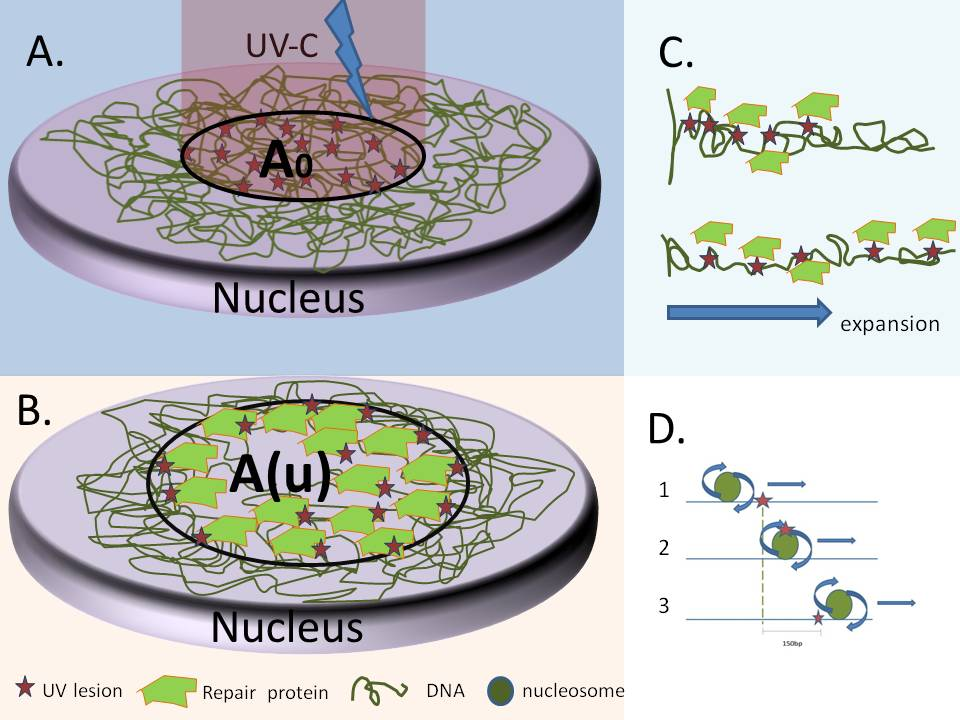
\includegraphics[width=0.7\linewidth, height=0.4\textheight]{ExperimentalProcedure}
			\caption{\small{\textbf{Expansion of the ROI post UV-C as a result of chromatin de-compaction and nucleosome sliding.} \textbf{A.} illumination of UV-C (red cylinder) in the initial damage region (DR) of area $A_0$ create uniformly distributed UV lesions (red stars) shows repair proteins (green polygons) de-compact the chromatin to access DNA damages. Additionally, to facilitate efficient repair, DNA is exposed by sliding nucleosomes. Chromatin de-compaction and nucleosome sliding expand the DR up to a maximal area $A(u)$ (the ROI), reached 15 minutes post UV-C irradiation \textbf{C.} expansion of the DR due to DNA de-compaction by chromatin remodlers and repair proteins results in equal proportion of DNA and nucleosome signal extrusion from the ROI \textbf{D.} nucleosome sliding allows additional loss of nucleosome signal with no DNA signal loss. Three time points on a 1D representation shows the principle of nucleosome signal loss with no DNA signal loss from the ROI. Nucleosomes (green circle) slide over a UV lesion (red star) displaces the lesion spatially by a distance equivalent to length of DNA wrapped on a histone ($\approx150 bp$) }. As nucleosome slide, tagged repair protein will bind to newly exposed damage points, thus expanding the DR while retaining all UV lesions in it.}
			\label{fig:ExperimentalProcedure}
		\end{figure}
		
	Experimental data shows a higher proportion of nucleosome signal loss than DNA for all UV dose (Figure \ref{fig:histoneAndDnaVsUvDoseModelFit}). To explain this observation we assume that the loss of DNA and nucleosome signals post UV-C is due to two mechanisms: the first is chromatin expansion, and the second is nucleosomes sliding along the chromatin. 
	
	For chromatin expansion, recruitment of repair and chromatin remodeling factors to bind to damaged DNA causes chromatin de-compaction and cross-links break to facilitate efficient repair \cite{gaillard2003chromatin,luijsterburg2012ddb2,deem2012epigenetic}. Accumulation of repair factors in the DR will generate a pushing force on surrounding chromatin in a radial outward direction \cite{dinant2007activation}. As a result, DNA and nucleosome outside the DR will be extruded from the ROI in equal proportions (Figure \ref{fig:ExperimentalProcedure} box A-C).
	
	An additional proportion of nucleosome signal loss is caused by the mechanism of nucleosome sliding. This mechanism allows nucleosome signal loss with no additional DNA signal loss. Repair proteins slide nucleosomes wrapped by damaged DNA away from high concentration of DNA damages to expose damaged DNA \cite{gaillard2003chromatin}. As a result the chromatin in the DR will loosen and remodeling and repair proteins will bind to the exposed damaged sites. This further contribute to the pushing of undamaged DNA outside the DR while retaining damaged DNA within it (Figure \ref{fig:ExperimentalProcedure} box D).  

    In-line with the description above, we construct a model representing
	signal loss 15 minutes post UV-C as a function of the UV dose. We do not take into account the
	mechanism of signal loss in time and only present equations representing the maximal loss of signal 15 minutes post UV-C.
	

	\subsection{Dynamics of DNA and nucleosome loss from the DR}
	The DR and the ROI are considered to be two-dimensional concentric circular regions, characterized by an area $A_0$ and $A(u)$, respectively. We assume an initial uniform distribution of DNA in the DR and its vicinity, such that the amount of DNA in $A(u)$ is $c_dA(u)$, with $c_d$ in units of $bp/\mu m^2$. 
	
	We restrict DNA damages to be inflicted only in $A_0$ immediately after UV induction. We set $T(u)$ to represent the amount of damaged DNA left in $A(u)$ 15 minutes post UV-C, while the undamaged DNA is assumed to be extruded. Therefore, the fraction of DNA signal loss, $D(u)$, is calculated as the ratio of extruded DNA to the total amount of DNA in the ROI, $c_dA(u)$. 
	\begin{equation}\label{eq:DNALossFraction}
	D(u) = \frac{c_dA(u)- T(u)}{c_dA(u)}
	\end{equation}
	
	We set the number of nucleosomes in a $A(u)$ to be $c_nA(u)$, with $c_n$ a constant in units of $nucleosomes/\mu m^2$. The total fraction of nucleosome extruded from the ROI, $H(u)$, is calculated as the sum of nucleosomes extruded along with undamaged DNA and the ones sliding out.
	\begin{equation}\label{eq:nucleosomeLossFraction}
	H(u) = D(u) + \frac{N_S(u)}{c_nA(u)}	
	\end{equation}
	
	In order to evaluate the fractions in \eqref{eq:DNALossFraction} and \eqref{eq:nucleosomeLossFraction}, we shall first formulate a model for the damaged DNA in the DR, $T(u)$ and derive $A(u)$ and $N_S(u)$ based on it.
	
	\subsection{DNA damages in the DR as a function of the UV dose}\label{subsection:AccumulationOfDNADamagesInTheDR}
	 We assume a uniform illumination of the UV in $A_0$ such that the average number of damages per $\mu m^2$ is constant for a fixed $u$ . As the UV exposure time increases, we assume that the average number of damages per $\mu m^2$ increases as $k_tu$, with $k_t$ in units of $bp/(msec\times \mu m^2)$. Because no two damages can occur on the same position on the DNA, the rate of accumulation of DNA damages with UV dose can be written as
	\begin{equation}\label{eq:DNADamageRate}
	\frac{dT(u)}{du} = k_tu(c_dA_0 - T(u))
	\end{equation}	
	 Using the initial condition $T(0) = 0$, the solution to equation \eqref{eq:DNADamageRate} is
	\begin{equation}\label{eq:DNADamageDR}
		T(u) = c_dA_0(1-\exp(-k_tu^2))
	\end{equation}
	
	\subsection{The number of nucleosomes sliding out of the DR}
	We now turn to construct a model for the number of nucleosomes $N_S(u)$
	sliding out of the DR and subsequently out of the ROI as a function of the UV dose. Although the exact mechanism by which nucleosome are lost is not known, 
	we propose that the rate of nucleosomes sliding out is proportional to the fraction of nucleosomes affected by increase of UV dose in $A_0$. In the first-order approximation, the dynamics of nucleosomes sliding is given by
	\begin{equation}\label{eq:nucleosomeSlideRate}
	\frac{dN_S(u)}{du} = k_s\left(c_nA_0-N_S(u))\right)\frac{dT(u)}{du}	 
	\end{equation}
	with $k_s$ a constant of units $1/bp$. Using the initial condition $N_S(0)=0$, the solution to equation \eqref{eq:nucleosomeSlideRate} is 
	\begin{equation}\label{eq:nucleosomeSlideDR}
	N_S(u)= c_nA_0\left(1-\exp(-k_sT(u))\right)
	\end{equation}
	with $T(u)$ defined in equation \eqref{eq:DNADamageDR}.
   \subsection{The ROI expansion}
	Next, we model the dynamics of the ROI area $A(u)$ with increasing UV
	dose. For this end, we consider the ROI area to expand as a result of the de-compaction of the damaged DNA, and by the effect of nucleosome sliding. 			
	\begin{equation}\label{eq:RoiAreaGrowthRate}
	\frac{dA(u)}{du}=k_a\frac{dN_S(u)}{du}+k_b\frac{dT(u)}{du}
	\end{equation}
	where $k_a$ is a constant of units $\mu m^2/ nucleosomes$ and $k_b$ of units $\mu m^2/ bp$. Using the initial condition $A(0) = A_0$, the solution to equation \eqref{eq:RoiAreaGrowthRate} is
	\begin{equation}\label{eq:RoiArea}
	A(u) = A_0+ k_ac_nA_0\left(1-\exp(-k_sT(u))\right)+k_bT(u)
	\end{equation}
	 with $A_0$ representing the size of a DR even in the absence of UV irradiation.
	 
	 \subsection{Final expression for DNA $D(u)$ and nucleosome $H(u)$ signal loss}
	We can now substitute the functions \eqref{eq:DNADamageDR}, \eqref{eq:nucleosomeSlideDR}, \eqref{eq:RoiArea} into the equations \eqref{eq:DNALossFraction} and \eqref{eq:nucleosomeLossFraction} to get the expressions for $D(u)$ and $H(u)$. We present the result in terms of $T(u)$
	\begin{equation}\label{eq:DNALoss}
	D(u) = 1-\frac{1}{1+ k_ac_n\left(1-\exp(-k_sT(u))\right)+k_bT(u)/A_0} 
	\end{equation}
	\begin{equation}\label{eq:nucleosomeLoss}
		H(u) = 1- \frac{\exp(-k_sT(u))}{1+ k_ac_n\left(1-\exp(-k_sT(u))\right)+k_bT(u)/A_0}
	\end{equation}
	
	\subsection{Parameter fit for $D(u)$ and $H(u)$}\label{subsection:parameterFit}
     We simultaneously fit equations \eqref{eq:DNALoss}  and \eqref{eq:nucleosomeLoss} to the H3.3 and DNA loss data, with the goal of maximizing the $R^2$ of both equations. Excluding the measurement at 5 msec, and using classical fitting procedure, we find
	\begin{equation*}
	k_tA_0 = 8\times 10^{-4}, \quad k_sc_dA_0 = 0.31,\quad k_ac_n = 0.29, \quad k_bc_d = 0.24
	\end{equation*}
	with $R^2 = 0.94$ and $R^2 = 0.955$ for DNA and nucleosome loss fit respectively.
	
	
\begin{figure}[H]
\centering
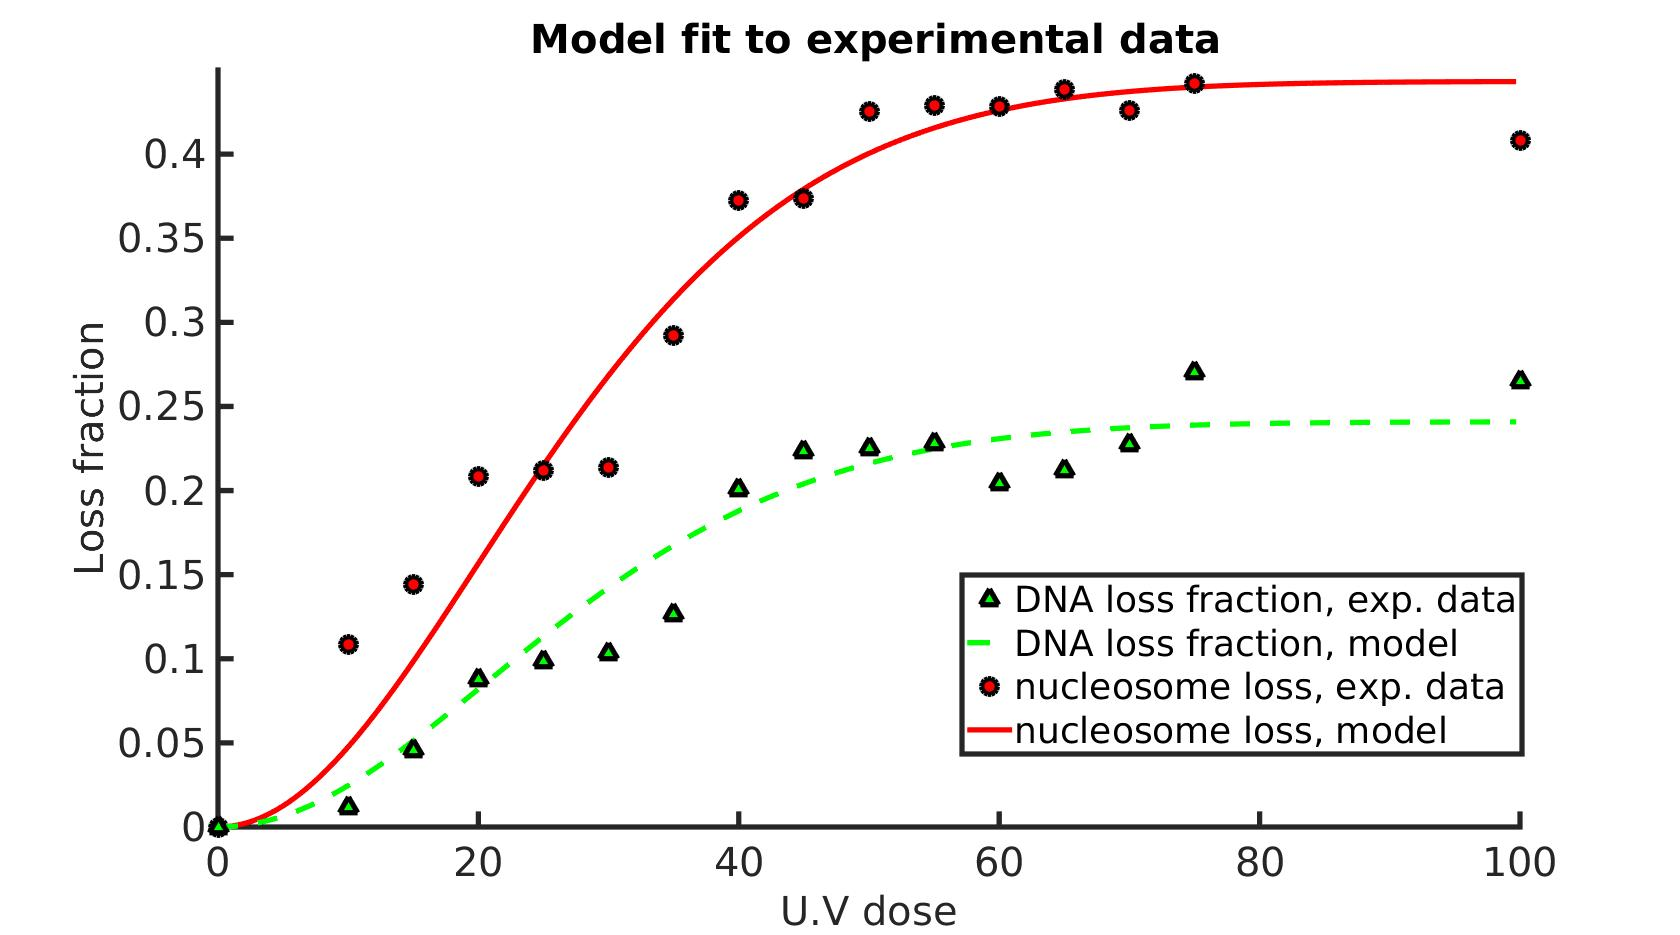
\includegraphics[width=0.5\linewidth, height=0.3\textheight]{histoneAndDnaVsUvDoseModelFit}
\caption{\textbf{Histone (red) and DNA (green) loss: experimental data
	for nucleosomes (circle) and DNA (triangles) versus model curves
	(continuous and dashed, respectively)}. Parameter values are obtained
	by simultaneously fitting equations\eqref{eq:DNALoss}  and \eqref{eq:nucleosomeLoss} to the experimental data with
	the goal of maximizing the $R^2$. The resulting curves show $R^2 = 0.94$ and
	$R^2 = 0.955$ for DNA and nucleosome loss, respectively.}
\label{fig:histoneAndDnaVsUvDoseModelFit}
\end{figure}

\subsection{Relative contribution of opening and sliding to DNA
	and nucleosome signal loss}

Using the calibrated model in equation equations \eqref{eq:DNALoss} and \eqref{eq:nucleosomeLoss}, we now calculate the
relative contribution of chromatin opening and nucleosome sliding to the
total loss of DNA and nucleosome signals. The sliding contribution refers to all loss
caused by either directly sliding nucleosome out of the DR or as the effect
nucleosome sliding has on pushing chromatin out of the DR. Chromatin opening contribution refers to all signal loss caused by chromatin remodeling.

We start by partitioning equation \eqref{eq:RoiArea}, describing the ROI into the two sub-mechanisms contributing to its expansion 
\begin{equation*}
A(u) = A_P(u) +A_S(u)
\end{equation*}
with $A_P(u)=A_0+k_bT(u)$, the area attributed to chromatin opening, and $A_S(u)=k_aN_S(u)$ to nucleosome sliding. 

The fraction of DNA signal loss attributed to chromatin opening is calculated similarly to equation \eqref{eq:DNALossFraction} as 
\begin{equation*}
D_P(u)=\frac{c_dA_P(u)-c_dA_0}{c_dA(u)}
\end{equation*}
The relative contribution of chromatin opening to the total DNA signal loss is therefore,
\begin{equation}\label{eq:relativeOpeningDNA}
\frac{D_P(u)}{D(u)}=\frac{A_P(u)/A_0-1}{A(u)/A_0-1}
\end{equation}	
The relative contribution of nucleosome sliding to the total DNA signal loss is
\begin{equation}\label{eq:relativeSlidingDNA}
\frac{D_S(u)}{D(u)}=1-\frac{D_P(u)}{D(u)}
\end{equation}

The relative contribution of chromatin opening and nucleosome
sliding to the total nucleosome signal loss is given respectively by
\begin{eqnarray}
\frac{H_P(u)}{H(u)} &=& \frac{D_P(u)}{H(u)}\label{eq:relativeOpeningNucleosomes}\\
\frac{H_S(u)}{H(u)} &=&1-\frac{H_P(u)}{H(u)} \label{eq:relativeSlidingNucleosomes}
\end{eqnarray}
where here we have used the fact that $H_P(u) = D_P(u)$, i.e fraction of nucleosomes extruded from the ROI along with undamaged DNA. Graphs of
equations \eqref{eq:relativeOpeningDNA}-\eqref{eq:relativeSlidingNucleosomes} are presented in Figure \ref{fig:relatiiveContributionToLoss}.

% The bibliography
\bibliographystyle{plain}
\bibliography{MaterialsAndMethodsModel.bib} % the bibliography.bib file 

\end{document}